\section{Wprowadzenie do QNX Momentics}


%% W celu opracowania programów pracujących pod kontrolą systemu operacyjnego czasu rzeczywistego (hard real time), będziemy potrzebowali Platformy Programistycznej QNX. W jej skład wchodzi pakiet QNX Momentics Tool Suite, składający się z elementów niezbędnych do rozwoju i uruchomienia oprogramowania pod QNX Neutrino - patrz rysunek~\ref{fig:qnxMomentics}. Do tej grupy należą kompilatory, linker, biblioteki i~inne komponenty systemu operacyjnego, zbudowane dla wszystkich architektur wspieranych przez QNX Neutrino. Posługując się QNX Momentics w systemie operacyjnym Windows i~Linux mamy do dyspozycji zintegrowane środowisko programistyczne na bazie projektu Eclipse.
%% 
%% 
%% \begin{figure}[!h]
%% \centering
%% 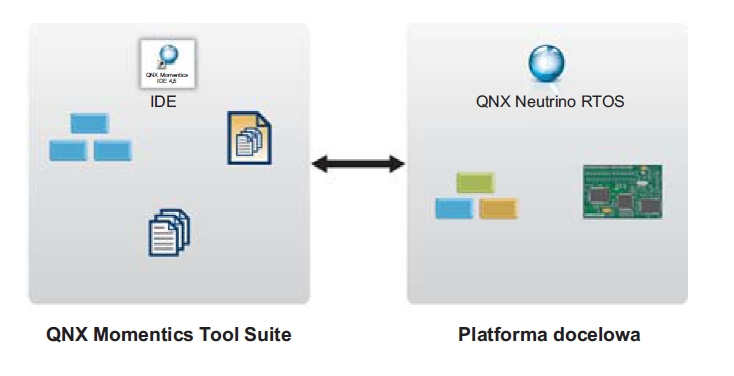
\includegraphics[width=0.35\textwidth]{img/qnxMomentics}
%% \caption{Platforma rozwoju oprogramowania}
%% \label{fig:qnxMomentics}
%% \end{figure}
%% 
%% Dzięki platformie programistycznej możemy tworzyć oprogramowanie w konfiguracji cross development (host-target). Na maszynie typu host (Windows) będziemy dysponować platformą programistyczną QNX Momentics, natomiast na maszynie docelowej typu target (QNX Neutrino na maszynie wirtualnej) będziemy uruchamiać nasze programy. Komunikacja pomiędzy komputerem host i target odbywa się przez sieć, a wspomaga go proces \lstinline[style=MyBashStyle]{qconn}.
%% 
%% \begin{figure}[!h]
%% \centering
%% 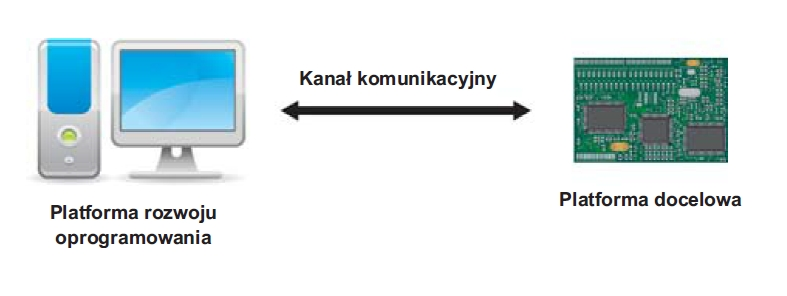
\includegraphics[width=0.5\textwidth]{img/konfiguracja}
%% \caption{Konfiguracja host-target}
%% \label{fig:konfiguracja}
%% \end{figure}
%% 
%% Niniejsze laboratorium będzie poswięcone kilka zagadnieniom:
%% \begin{myenumerate}
%% \item Podstawy obsługi QNX Momentics
%% \item Zarządzanie projektami C/C++
%% \item Edycja kodu źródłowego, kompilacja i~budowanie
%% \item Dostęp do platformy docelowej oraz uruchamianie aplikacji
%% \end{myenumerate}
%% 
%% 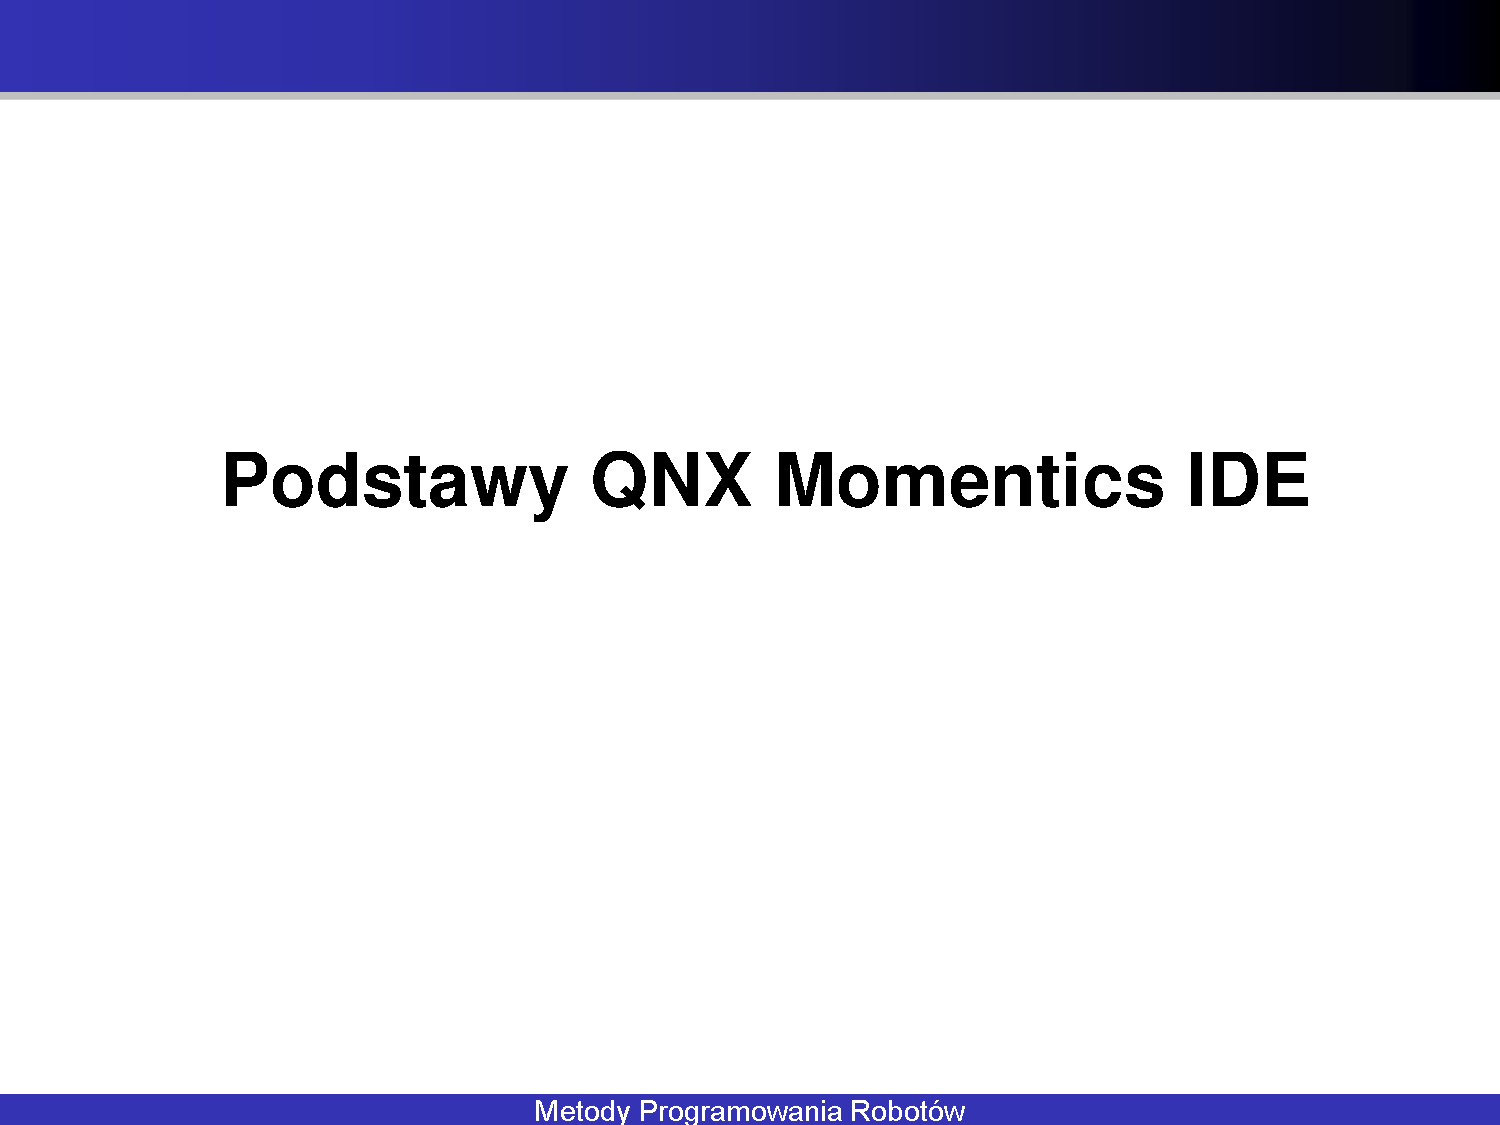
\includepdf[scale=0.75,pages={1-8},pagecommand={\thispagestyle{fancy}{\subsection{Podstawy obsługi QNX Momentics}}},nup=2x4]{img/qnx1.pdf}
%% \includepdf[scale=0.75,pages={9-},pagecommand={\thispagestyle{fancy}{}},nup=2x4]{img/qnx1.pdf}
%% 
%% 
%% 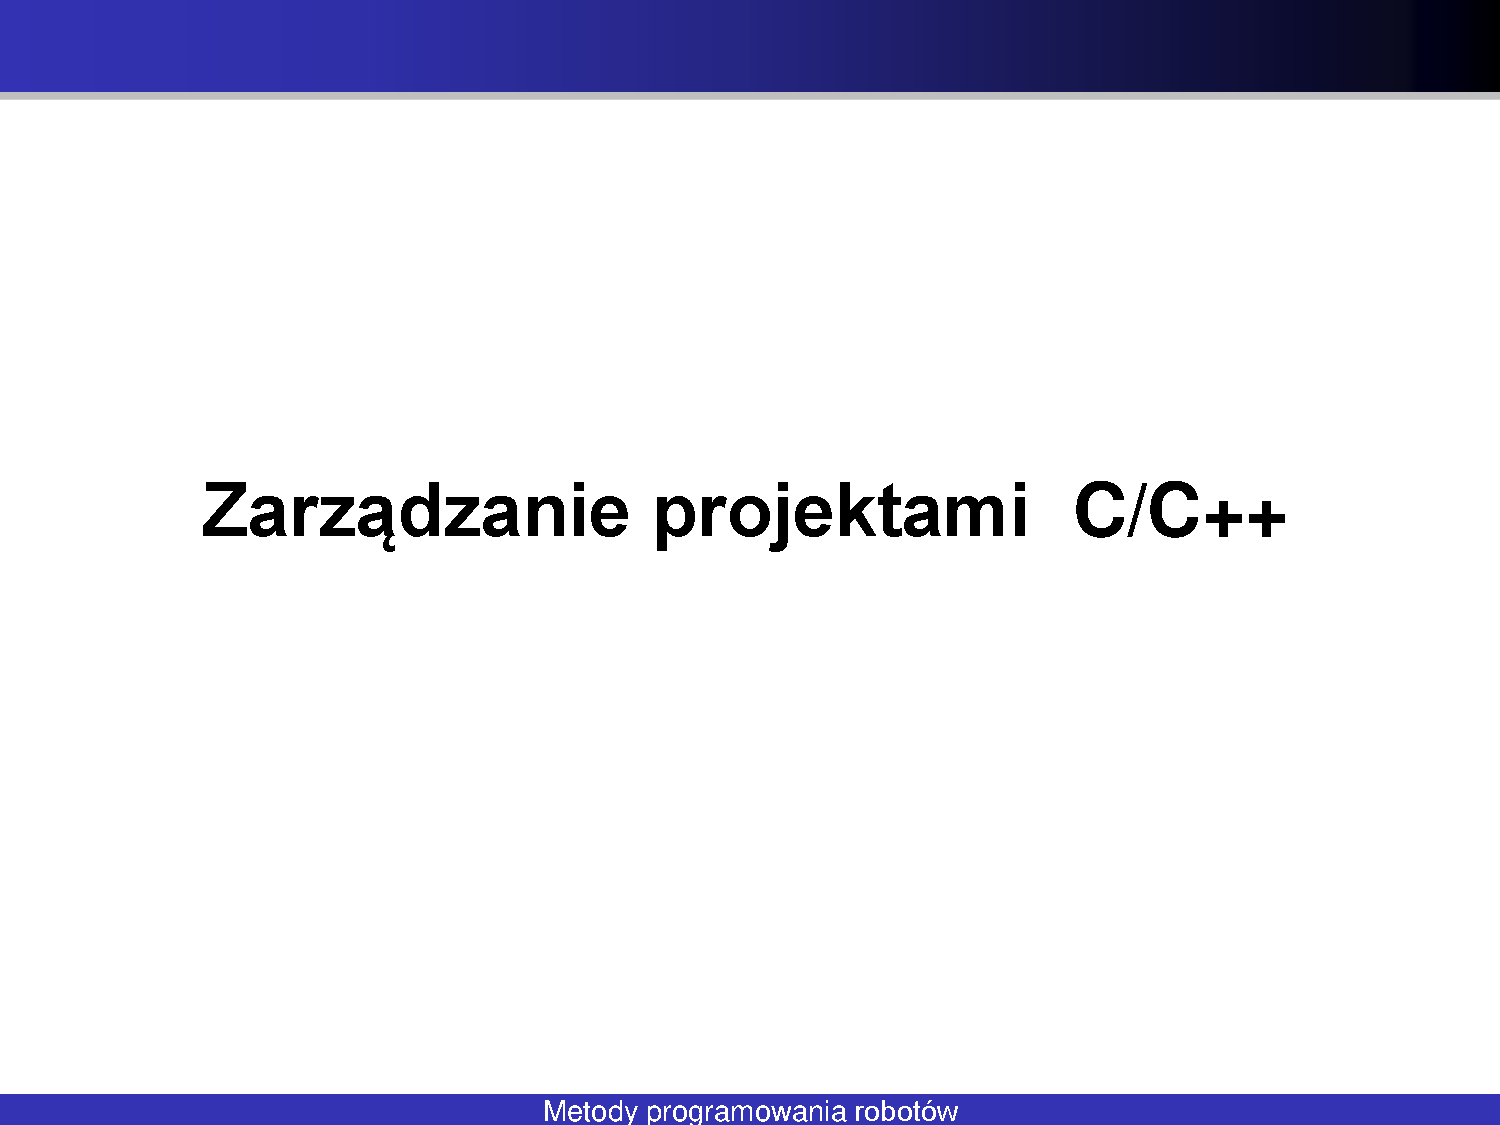
\includepdf[scale=0.75,pages={1-8},pagecommand={\thispagestyle{fancy}{\subsection{Zarządzanie projektami C/C++}}},nup=2x4]{img/qnx2.pdf}
%% \includepdf[scale=0.75,pages={9-},pagecommand={\thispagestyle{fancy}{}},nup=2x4]{img/qnx2.pdf}
%% 
%% 
%% 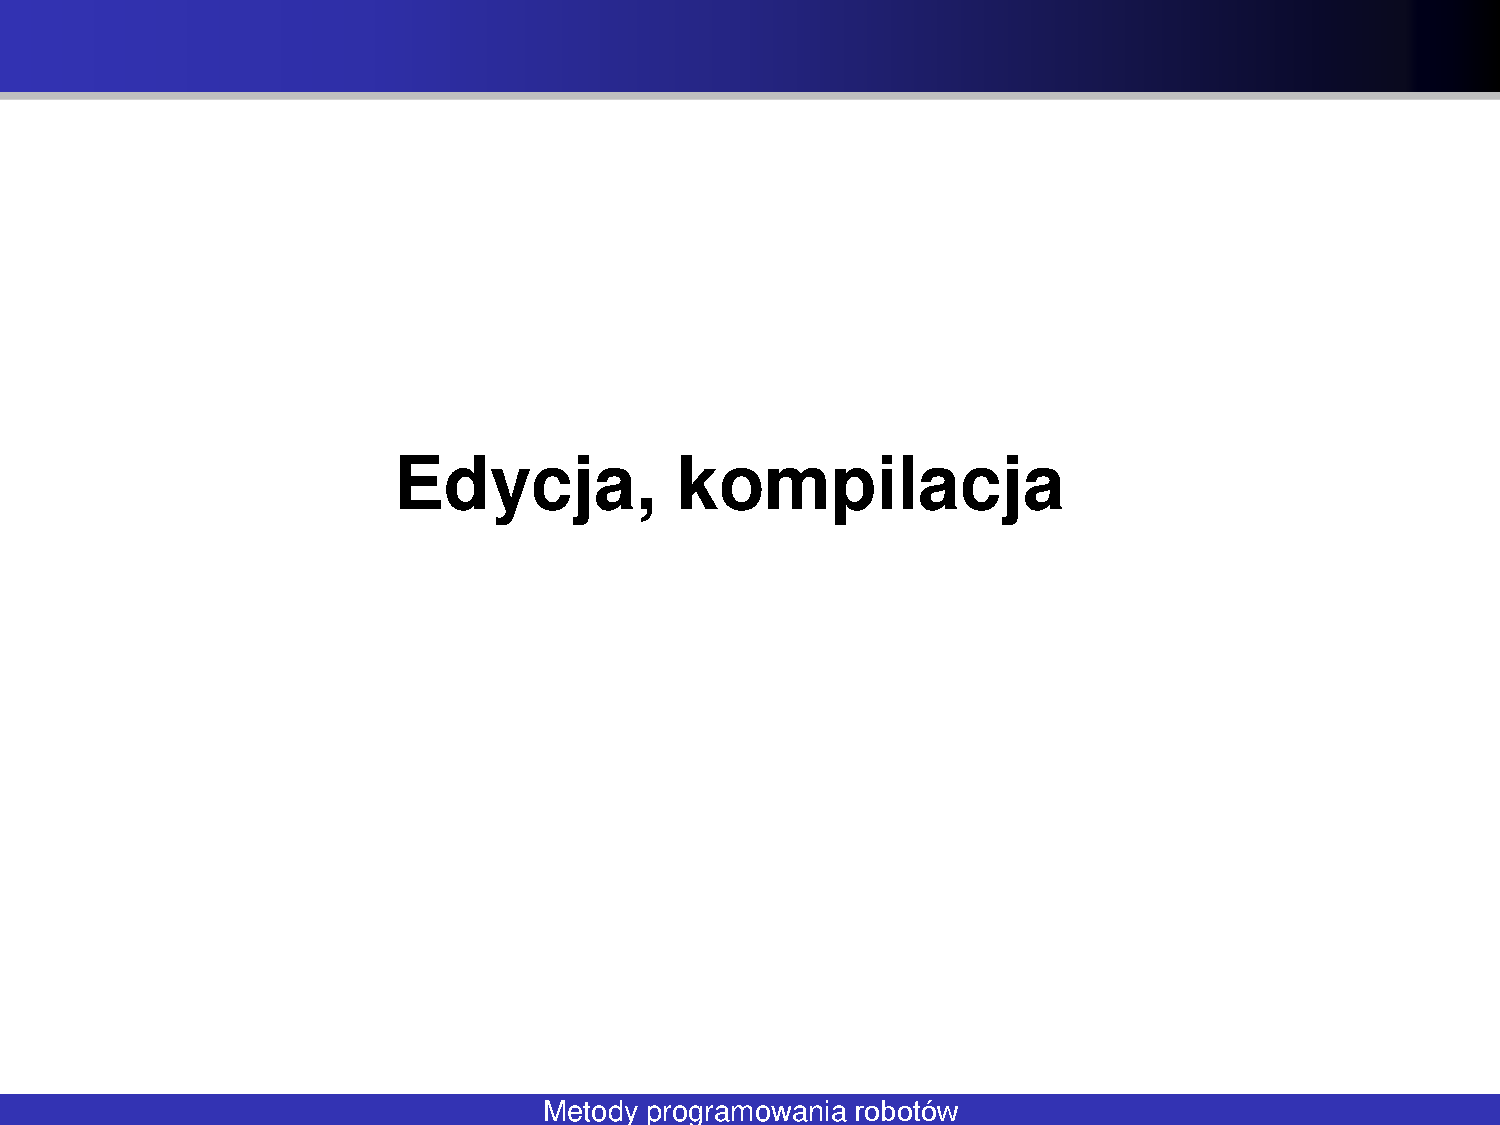
\includepdf[scale=0.75,pages={1-8},pagecommand={\thispagestyle{fancy}{\subsection{Edycja kodu, kompilacja i~budowanie}}},nup=2x4]{img/qnx3.pdf}
%% \includepdf[scale=0.75,pages={9-},pagecommand={\thispagestyle{fancy}{}},nup=2x4]{img/qnx3.pdf}
%% 
%% 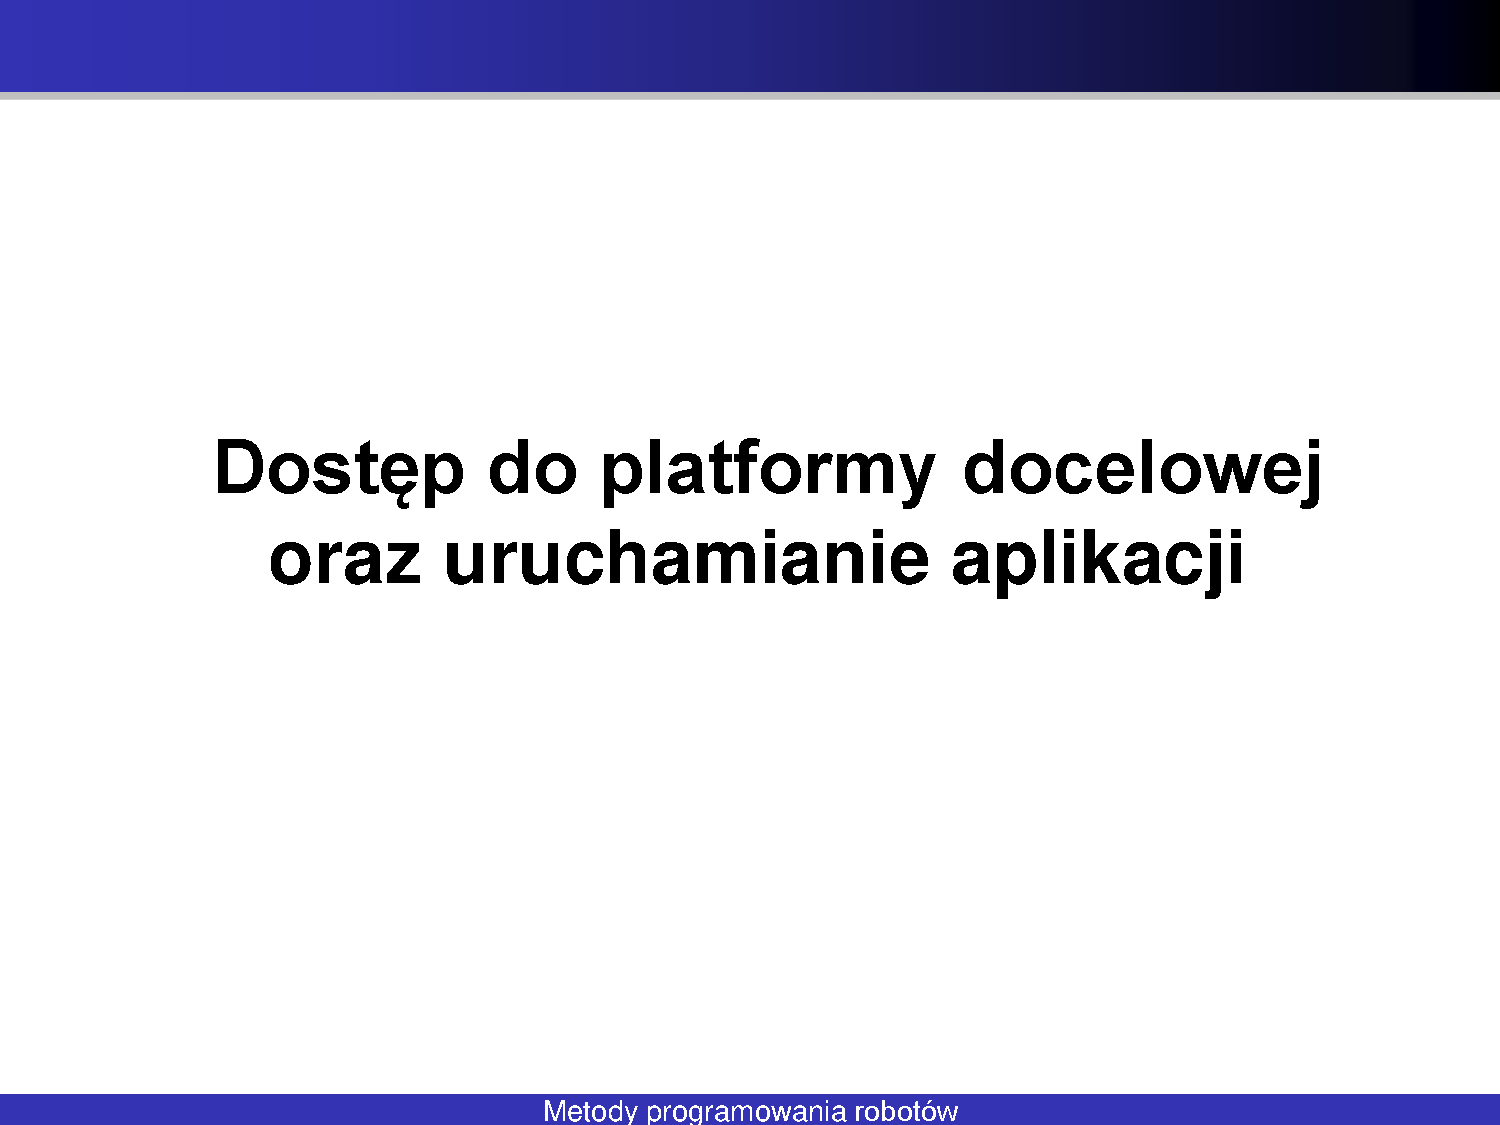
\includepdf[scale=0.75,pages={1-8},pagecommand={\thispagestyle{fancy}{\subsection{Dostęp do platformy docelowej oraz uruchamianie aplikacji}}},nup=2x4]{img/qnx4.pdf}
%% \includepdf[scale=0.75,pages={9-},pagecommand={\thispagestyle{fancy}{}},nup=2x4]{img/qnx4.pdf}
%% 
%% %\clearpage
%% %\phantomsection
%% %{\label{viRef}
%% %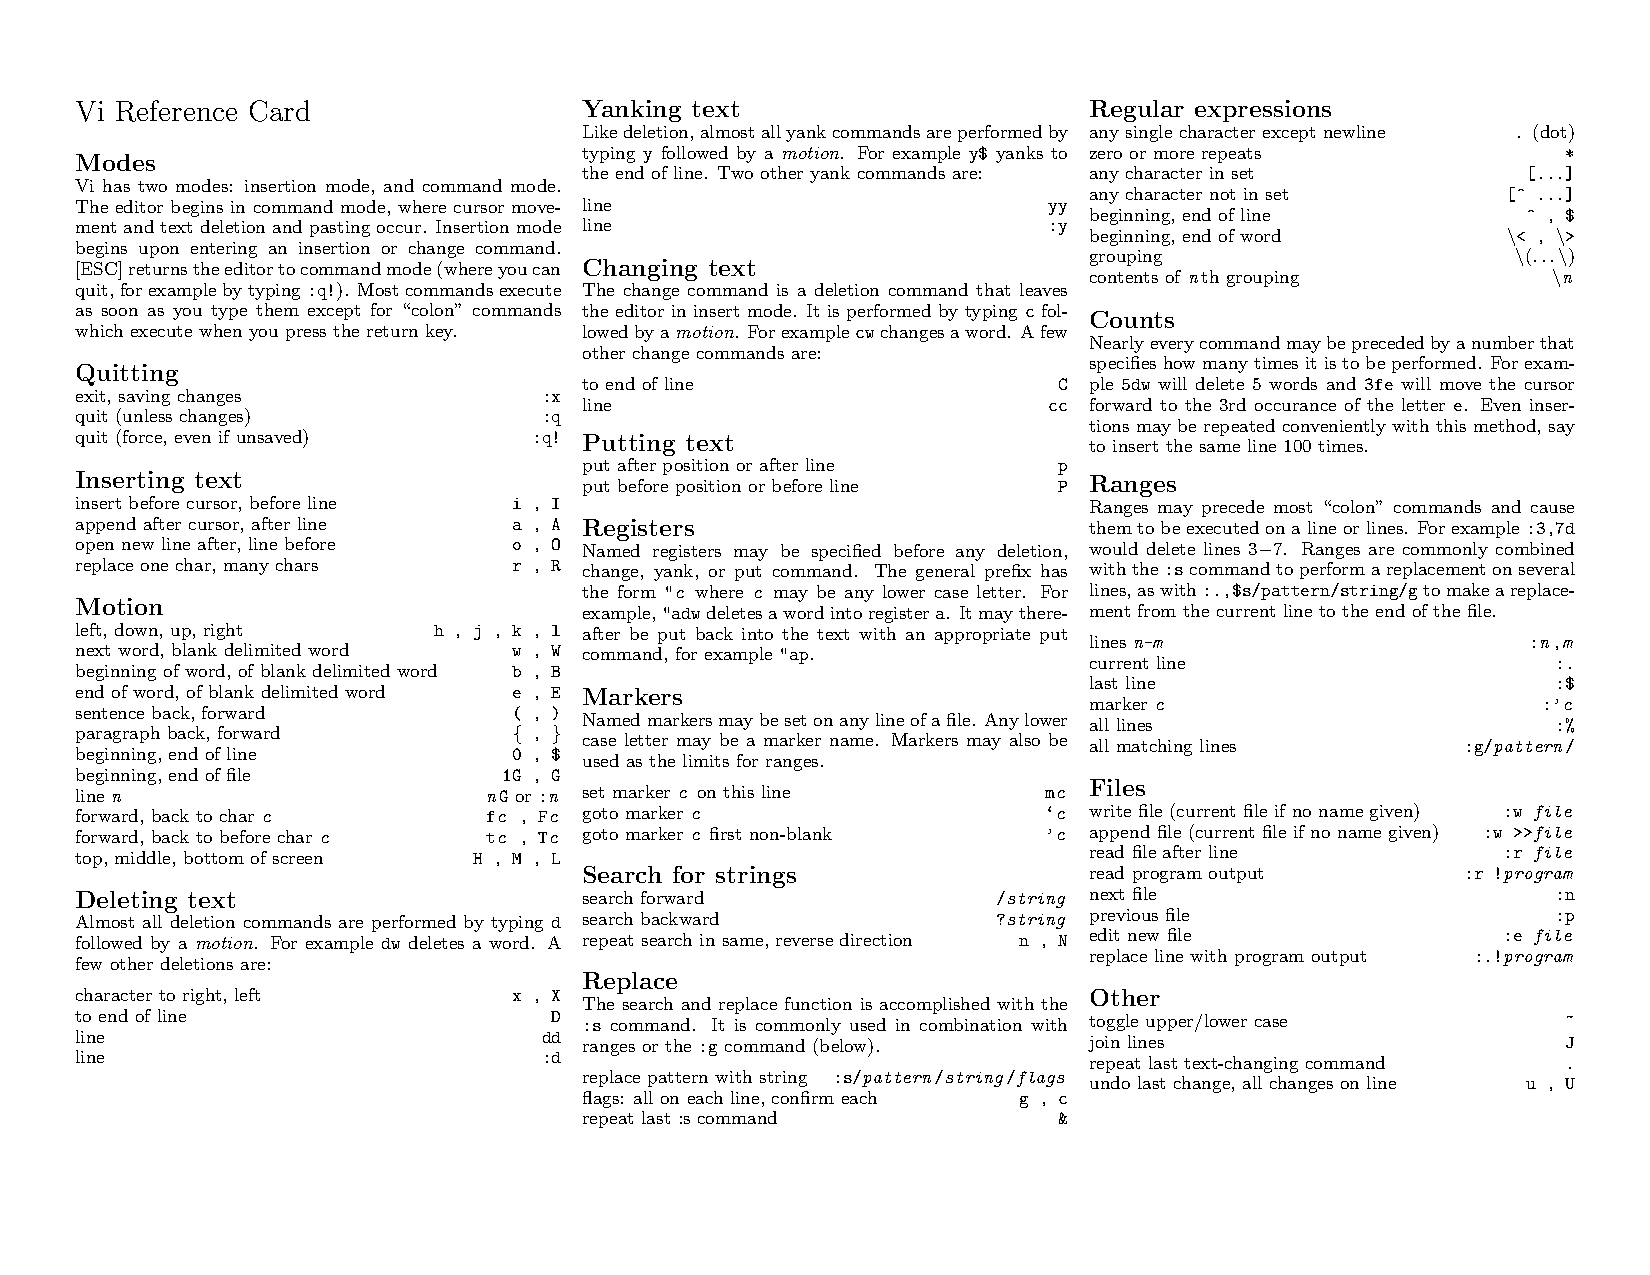
\includepdf[scale=0.95,pages={1},pagecommand={\thispagestyle{fancy}},pagecommand={\thispagestyle{fancy}{\label{subsec:vi}}},lastpage=1,angle=90]{img/viRef.pdf}
%% %}
%% 
%% %\subsection{Zarządzanie projektami C}
%% %
%% %\subsection{Edycja kodu źródłowego, kompilacja i~budowanie}
%% %
%% %\subsection{Dostęp do platformy docelowej oraz uruchamianie aplikacji}
%% %\subsection{Ćwiczenia}

\cleardoublepage
